\documentclass[border=10pt]{standalone}
\usepackage{tikz}
\usetikzlibrary{shapes.geometric, arrows, positioning, calc, fit, backgrounds}

% Use Atkinson Hyperlegible font
\usepackage[sfdefault]{atkinson}

% Define colors
\definecolor{boxcolor}{RGB}{200, 240, 240}
\definecolor{decisioncolor}{RGB}{255, 235, 200}
\definecolor{arrowcolor}{RGB}{100, 100, 100}

\begin{document}
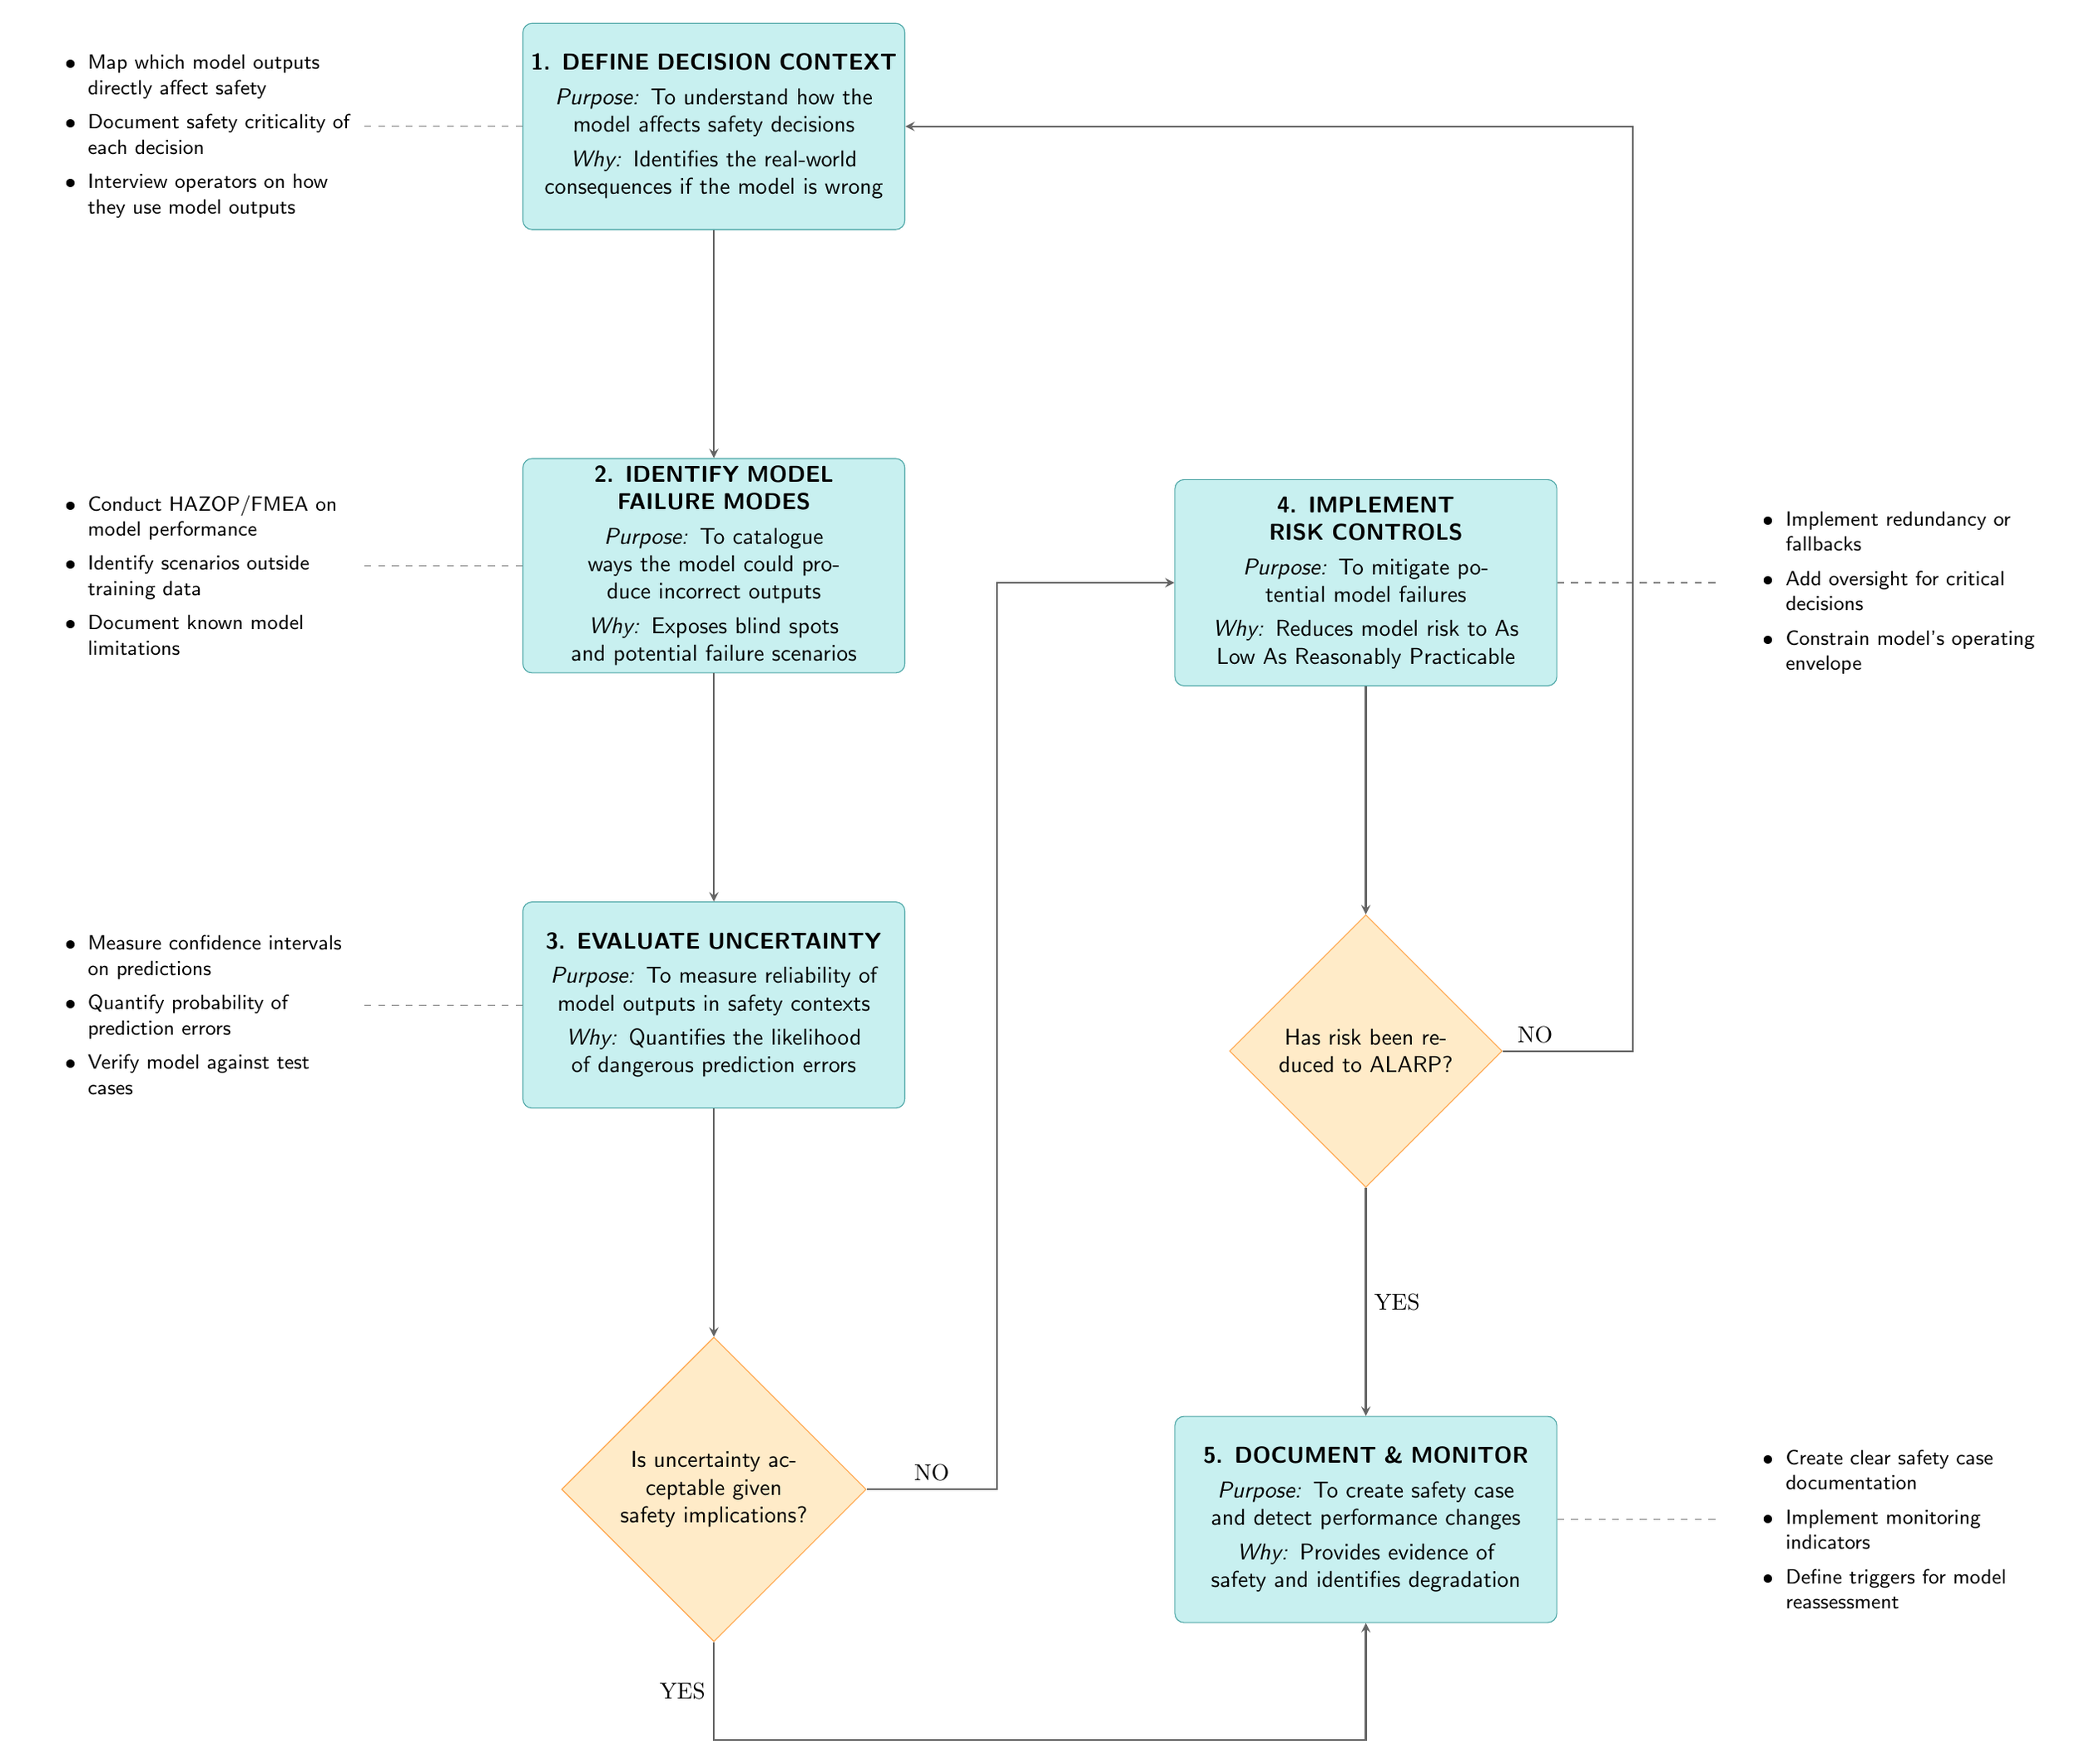
\begin{tikzpicture}[
    node distance=4cm,
    box/.style={
        rectangle, 
        rounded corners, 
        draw=teal!70, 
        fill=boxcolor, 
        text width=16em, 
        minimum height=9em, 
        align=center, 
        font=\sffamily
    },
    decision/.style={
        diamond, 
        draw=orange!70, 
        fill=decisioncolor, 
        text width=10em, 
        inner sep=0pt,
        align=center, 
        font=\sffamily
    },
    arrow/.style={
        thick, 
        -stealth, 
        draw=arrowcolor
    },
    connect/.style={
        dashed,
        draw=gray
    },
    tasklabel/.style={
        text width=14em,
        align=left,
        font=\sffamily\small
    }
]

% Create a coordinate system
\coordinate (origin) at (0,0);

% Main process nodes
\node[box] (step1) at ($(origin) + (8,0)$) {\textbf{1. DEFINE DECISION CONTEXT}\\[0.3em]
    \textit{Purpose:} To understand how the model affects safety decisions\\[0.3em]
    \textit{Why:} Identifies the real-world con\-sequences if the model is wrong};

\node[tasklabel, left=2.5cm of step1] (tasks1) {
    \begin{itemize}
        \item Map which model outputs directly affect safety
        \item Document safety criticality of each decision
        \item Interview operators on how they use model outputs
    \end{itemize}
};

\node[box, below=3.5cm of step1] (step2) {\textbf{2. IDENTIFY MODEL FAILURE MODES}\\[0.3em]
    \textit{Purpose:} To catalogue ways the model could pro\-duce incorrect outputs\\[0.3em]
    \textit{Why:} Exposes blind spots and potential failure scenarios};

\node[tasklabel, left=2.5cm of step2] (tasks2) {
    \begin{itemize}
        \item Conduct HAZOP/FMEA on model performance
        \item Identify scenarios outside training data
        \item Document known model limitations
    \end{itemize}
};

\node[box, below=3.5cm of step2] (step3) {\textbf{3. EVALUATE UNCERTAINTY}\\[0.3em]
    \textit{Purpose:} To measure reliability of model outputs in safety contexts\\[0.3em]
    \textit{Why:} Quantifies the likelihood of dangerous prediction errors};

\node[tasklabel, left=2.5cm of step3] (tasks3) {
    \begin{itemize}
        \item Measure confidence intervals on predictions
        \item Quantify probability of prediction errors
        \item Verify model against test cases
    \end{itemize}
};

% First decision diamond
\node[decision, below=3.5cm of step3] (decision1) {Is uncertainty acceptable given safety implications?};

% Right column nodes
\node[box] (step4) at ($(origin) + (18,-7)$) {\textbf{4. IMPLEMENT RISK CONTROLS}\\[0.3em]
    \textit{Purpose:} To mitigate po\-tential model failures\\[0.3em]
    \textit{Why:} Reduces model risk to As Low As Reasonably Practicable};

\node[tasklabel, right=2.5cm of step4] (tasks4) {
    \begin{itemize}
        \item Implement redundancy or fallbacks
        \item Add oversight for critical decisions
        \item Constrain model's operating envelope
    \end{itemize}
};

% Second decision diamond
\node[decision, below=3.5cm of step4] (decision2) {Has risk been reduced to ALARP?};

% Final step
\node[box, below=3.5cm of decision2] (step5) {\textbf{5. DOCUMENT \& MONITOR}\\[0.3em]
    \textit{Purpose:} To create safety case and detect performance changes\\[0.3em]
    \textit{Why:} Provides evidence of safety and identifies degradation};

\node[tasklabel, right=2.5cm of step5] (tasks5) {
    \begin{itemize}
        \item Create clear safety case documentation
        \item Implement monitoring indicators
        \item Define triggers for model reassessment
    \end{itemize}
};

% Connect task lists with dashed lines
\draw[connect] (step1.west) -- (tasks1.east);
\draw[connect] (step2.west) -- (tasks2.east);
\draw[connect] (step3.west) -- (tasks3.east);
\draw[connect] (step4.east) -- (tasks4.west);
\draw[connect] (step5.east) -- (tasks5.west);

% Main flow arrows
\draw[arrow] (step1.south) -- (step2.north);
\draw[arrow] (step2.south) -- (step3.north);
\draw[arrow] (step3.south) -- (decision1.north);

% Connect decision1 "NO" path to step4
\coordinate (decision1_right) at ($(decision1.east) + (2,0)$);
\draw[arrow] (decision1.east) -- node[above] {NO} (decision1_right) |- (step4.west);

% Connect decision1 "YES" path to step5
\coordinate (decision1_yes_path) at ($(decision1.south) + (0,-1.5)$);
\draw[arrow] (decision1.south) -- node[left] {YES} (decision1_yes_path) -| (step5.south);

% Flow within right column
\draw[arrow] (step4.south) -- (decision2.north);
\draw[arrow] (decision2.south) -- node[right] {YES} (step5.north);

% FIXED: Calculate the height difference first, then use it in coordinates
\path let \p1 = (step1.east), \p2 = (decision2.east) in coordinate (height_diff) at (0,\y1-\y2);

\coordinate (decision2_exit) at ($(decision2.east) + (2,0)$);
\coordinate (turn_point) at ($(decision2_exit) + (0,0)$);
\coordinate (high_point) at ($(turn_point) + (height_diff)$);

% Now draw the path with the precalculated coordinates
\draw[arrow] (decision2.east) -- node[above, near start] {NO} (decision2_exit) -- (turn_point) -- (high_point) -- (step1.east);

\end{tikzpicture}
\end{document}